\documentclass[12pt]{article}
\usepackage{caption}
\usepackage{graphicx, subfig}
\usepackage{float}
\usepackage{mathptmx}
\usepackage{graphicx}
\usepackage{listings}
\usepackage{amsmath}
\usepackage{amssymb}
\usepackage{algorithm}
\usepackage{color}

\definecolor{dkgreen}{rgb}{0,0.6,0}
\definecolor{gray}{rgb}{0.5,0.5,0.5}
\definecolor{mauve}{rgb}{0.58,0,0.82}

\lstset{frame=tb,
  language=Python,
  aboveskip=3mm,
  belowskip=3mm,
  showstringspaces=false,
  columns=flexible,
  basicstyle={\small\ttfamily},
  numbers=none,
  numberstyle=\tiny\color{gray},
  keywordstyle=\color{blue},
  commentstyle=\color{dkgreen},
  stringstyle=\color{mauve},
  breaklines=true,
  breakatwhitespace=true,
  tabsize=3
}
\title{Exploration 2}
\author{Student Name: Fanjie Kong
\\
Student ID: 2462691 }

\begin{document}
\maketitle
\newpage
\textbf{Integrate-and-fire model}
\\\\

1. Compute the firing-rate as a function of the applied input current for the exponential integrate-and-fire model.
\\

\textbf{Answer:} 
\\

I think the reason for staircase curve of firing rate is that in some case the reset operation may not happen because the high 'v' makes the $dv/dt$ negative enough to decrease the 'v' itself. 

 \begin{figure}[H]
  \centering
  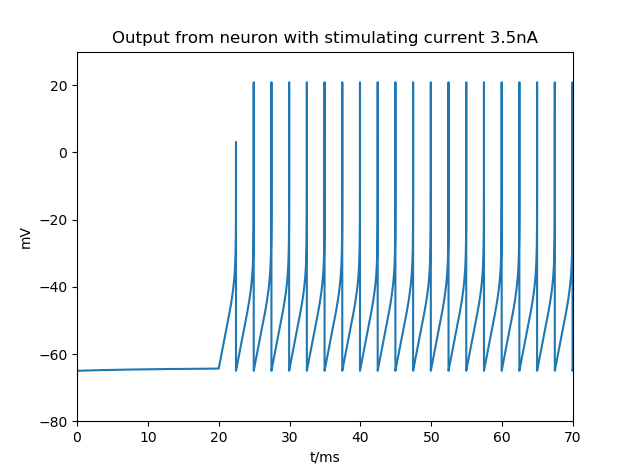
\includegraphics[width=.8\textwidth]{h2_p1_p1.png} %1.png是图片文件的相对路径
  \label{img} %此处的label相当于一个图片的专属标志,目的是方便上下文的引用
  \caption{Result 1.1}
\end{figure}

 \begin{figure}[H]
  \centering
  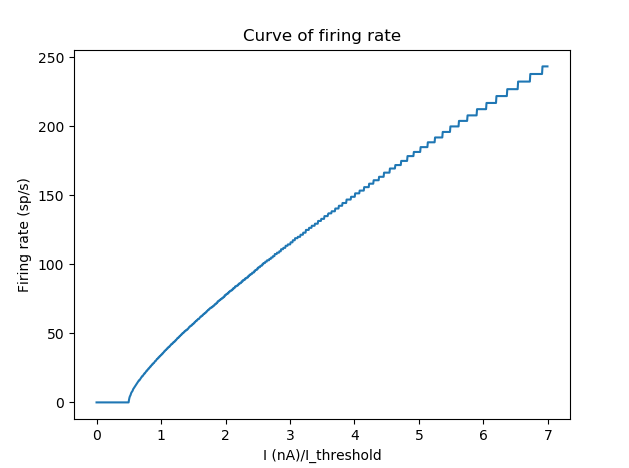
\includegraphics[width=.8\textwidth]{h2_p1_2.png} %1.png是图片文件的相对路径
  \label{img} %此处的label相当于一个图片的专属标志,目的是方便上下文的引用
  \caption{Result 1.2}
\end{figure}
 
\newpage
\textbf{Izhikevich model}
\\

Using the information on http://www.izhikevich.org/publications/spikes.htm (see Exploration 2 Links on sakai), implement the Izhikevich model in Brian 2. Try to reproduce 4 of the models with the proper choices of parameters. 
\\

\textbf{Answer:} 
\\

Regular Spiking has obviously frequency adaptation due to increasing u.
\begin{figure}[H]
\centering
    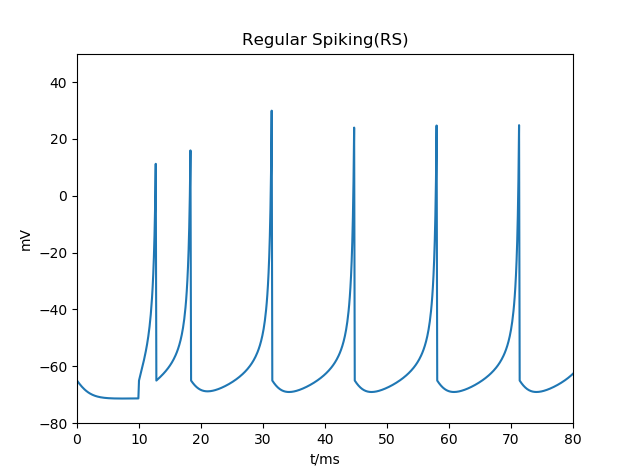
\includegraphics[width=.8\textwidth]{h2_p2_RS.png} %1.png是图片文件的相对路径
  \label{img} %此处的label相当于一个图片的专属标志,目的是方便上下文的引用
  \caption{Result 2.1}
\end{figure}

Because of higher c compared to RS, there are initially bursting in IB model, but it switches to spiking due to increasing u.
 \begin{figure}[H]
  \centering
    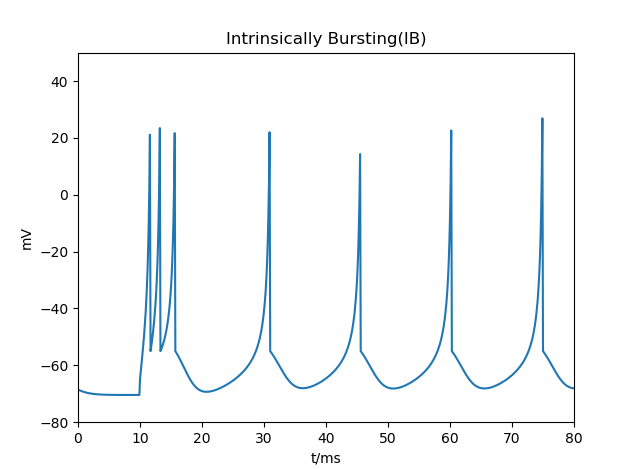
\includegraphics[width=.8\textwidth]{h2_p2_IB.png} %1.png是图片文件的相对路径
           \caption{Result 2.2}
           
Much higher 'a' causes the fast spiking with little frequency adaptation.

      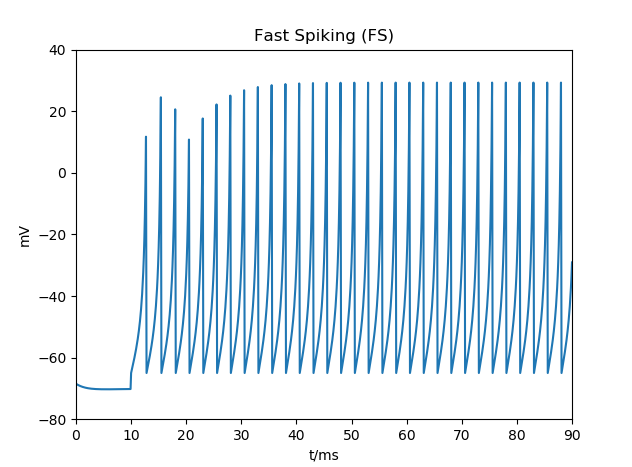
\includegraphics[width=.8\textwidth]{h2_p2_FS.png} %1.png是图片文件的相对路径
       \caption{Result 2.3}
  \label{img} %此处的label相当于一个图片的专属标志,目的是方便上下文的引用
\end{figure}

Due to much higher 'c'(-50 mV), there are bursting in CH model. And after bursting, 'u' becomes large, so there are spiking-jump.

 \begin{figure}[H]
  \centering
   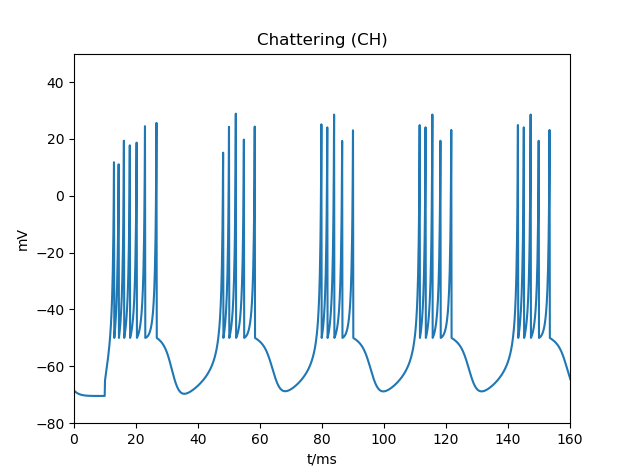
\includegraphics[width=.8\textwidth]{h2_p2_CH.png} %1.png是图片文件的相对路径
         \caption{Result 2.4}
  \label{img} %此处的label相当于一个图片的专属标志,目的是方便上下文的引用
\end{figure}
\newpage
\textbf{Alpha Conductance and Biophysical Model }
\\

1.  Using $synalpha_skel2018.py$ create a model of alpha synapse conductance and the 4 biophysical synapses conductances and modify the parameters to give a reasonable match to the 4 biological conductance changes driven by the 1 msec pulse signifying transmitter release. For NMDA- assume $B(V)= 1$. You will use the two odes to generate the alpha functions. The expressions for the conductance changes for the various biophysical synapses can be found in Chapter 8 of "Foundations of (Mathematical) Neuroscience" in the Relevant Online Texts section under Resources in Sakai. For which biophysical models does the alpha synapse conductance best compare? What biophysical models are not fit well with the alpha synapse conductance. 
\\

\textbf{Answer:} 
\\

Best compare:
AMPA, NMDA and GABAa model. These three model have the same formula format but different parameters.

Fit bad:
GABAb model. Due to the influence of 'r', GABAb needs more time to rise, so the alpha synapse cannot fit well in this situation. 

And what's interesting is that if we do not reset r or s for GABAb model when spiking comes, the two peak values for the conductance are not the same.
 \begin{figure}[H]
  \centering
  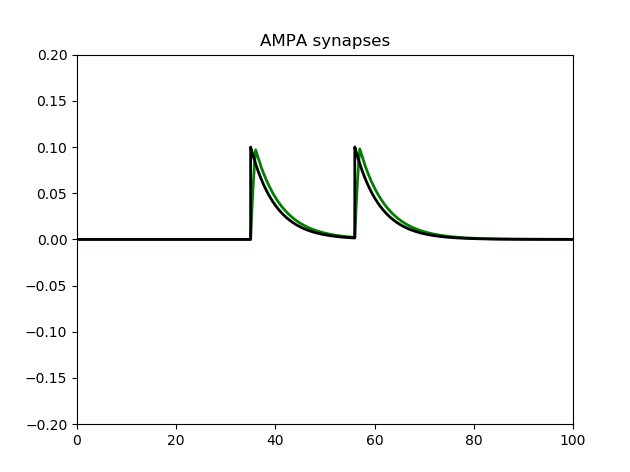
\includegraphics[width=.8\textwidth]{h2_p1_AMPA.png} %1.png是图片文件的相对路径
  \label{img} %此处的label相当于一个图片的专属标志,目的是方便上下文的引用
  \caption{Result 3.1}

\end{figure}
 \begin{figure}[H]
  \centering
    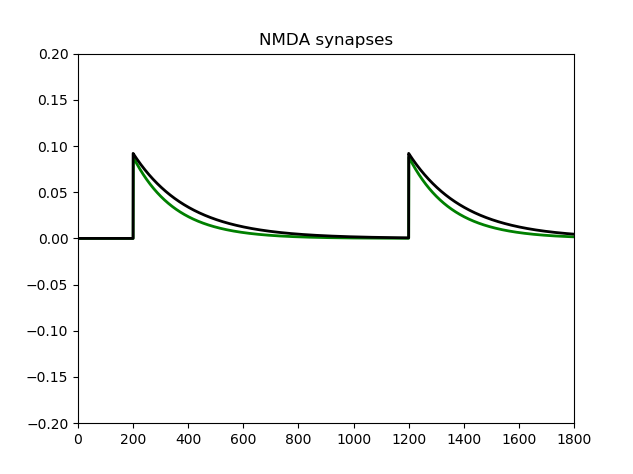
\includegraphics[width=.8\textwidth]{h2_p1_NMDA.png} %1.png是图片文件的相对路径
     \caption{Result 3.2}
      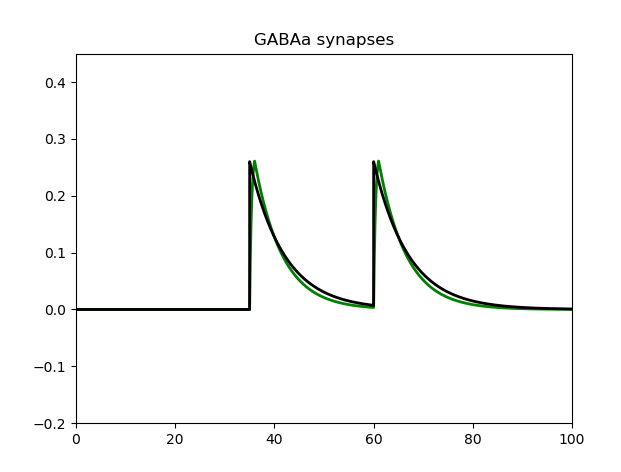
\includegraphics[width=.8\textwidth]{h2_p1_GABAa.png} %1.png是图片文件的相对路径
  \caption{Result 3.3}

\end{figure}

 \begin{figure}[H]
  \centering
        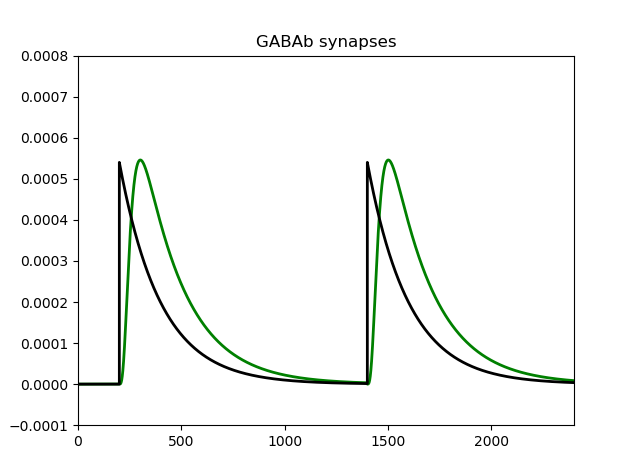
\includegraphics[width=.8\textwidth]{h2_p1_GABAb_2.png} %1.png是图片文件的相对路径
  \label{img} %此处的label相当于一个图片的专属标志,目的是方便上下文的引用
  \caption{Result 3.4}

\end{figure}

 \begin{figure}[H]
  \centering
        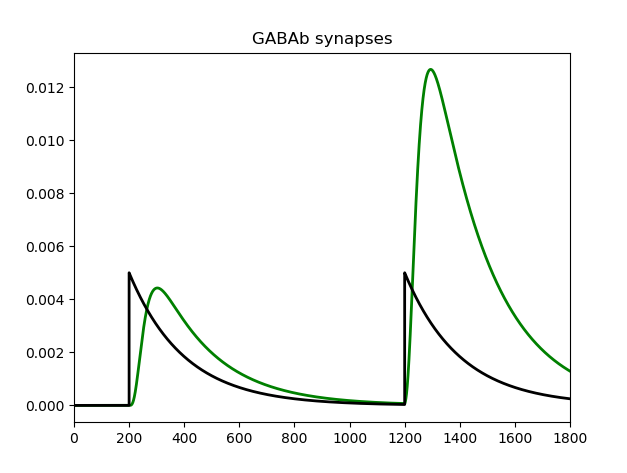
\includegraphics[width=.8\textwidth]{h2_p1_GABAb.png} %1.png是图片文件的相对路径
  \label{img} %此处的label相当于一个图片的专属标志,目的是方便上下文的引用
  \caption{Result 3.5}

\end{figure}

\newpage

2.A paper was uploaded to the sakai site under Task 2 - Synapses called “Modeling Synapses” by Roth and van Rossum. This paper gives a modified form for the two odes – namely 
 
$$ g= dg/dt =
−g/\tau_{decay}
+z(t)$$
 
$$ z= dz/dt =
−z/tau_{rise}
+g_{syn2}u(t)$$
 
where you can separately define the rise time constant and decay time constant. Adjust your code for Part B and play with the parameters $\tau_{rise}$  and $\tau_{decay}$ to see how this affects the shape of the conductance and the comparisons to the biophysical models for which the alpha model did not fit well. 
 
Here you should be aware that the conductance peaks at 
 
$$peaktime $$

\textbf{Answer:} 
\\

$\tau_{rise}$ represents the time for conductance rising when spiking comes. Increasing the $\tau_{rise}$ will prolong the rising time and vice versa. 
\\

$\tau_{decay}$ represents the time for conductance falling when spiking comes. Increasing the $\tau_{rise}$ will prolong the decay time and vice versa. 

 \begin{figure}[H]
  \centering
  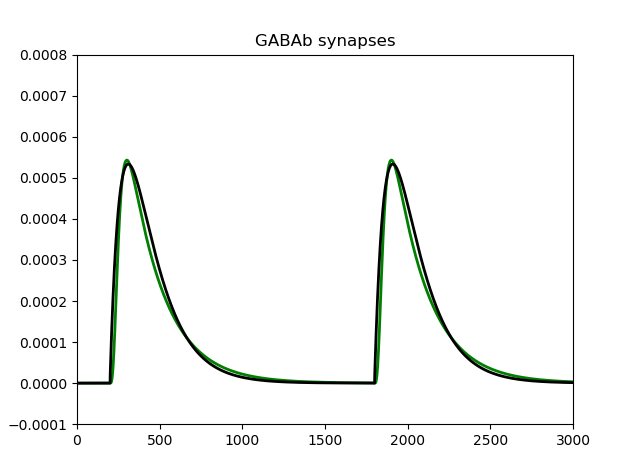
\includegraphics[width=.8\textwidth]{h2_p2_2_GABAb_fixed2.png} %1.png是图片文件的相对路径
   %1.png是图片文件的相对路径
  \label{img} %此处的label相当于一个图片的专属标志,目的是方便上下文的引用
  \caption{Result 4.1}
\end{figure}
\begin{figure}[H]
  \centering
  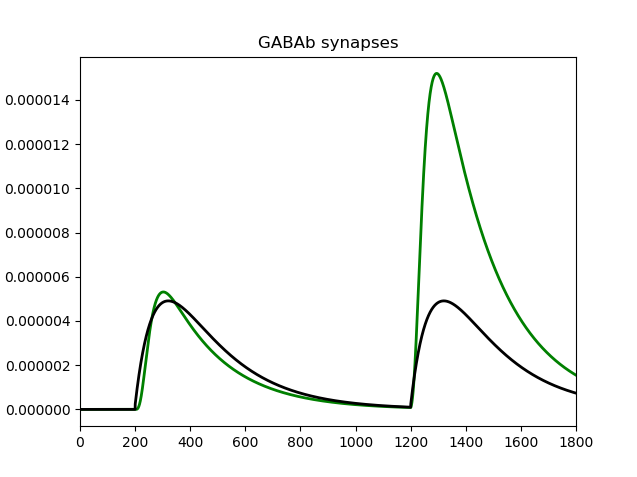
\includegraphics[width=.8\textwidth]{h2_p2_2_GABAb_fixed.png} %1.png是图片文件的相对路径
   %1.png是图片文件的相对路径
  \label{img} %此处的label相当于一个图片的专属标志,目的是方便上下文的引用
  \caption{Result 4.1}
\end{figure}

\newpage
\large \textbf{Appendix}
\\

\normalsize\textbf{EIAF}
\\

\lstset{language=Python}
\begin{lstlisting}
from brian2 import *
defaultclock.dt=.0005*ms
num_neurons = 100
duration = 20*ms
# Parameters
# area=20000*umetre**2 no more area for the neuron, the IAF model represents point(no area) neuron.
El = -65*mV
V_reset = -65*mV
V_th = -50*mV
tau_m = 10*ms
R_m = 10*Mohm
delta_e = 5.0*mV
VT = -55*mV
V_max = 30*mV



#The model
eqs_fv = '''
fv = delta_e * exp((v-VT)/delta_e) : volt
 '''


eqs = '''
d = El - v + fv + R_m*I : volt
dv/dt = (El - v + fv + R_m*I)/tau_m :  volt
I : amp
'''
eqs += (eqs_fv)

# Threshold and refractoriness are only used for spike counting
group = NeuronGroup(num_neurons, eqs,clock=Clock(defaultclock.dt),
                    threshold='v >= V_max',
                    reset='v=V_reset',
                    method='euler')
monitor2=StateMonitor(group, ('v', 'd',),  record=True)
group.v = -65*mV

group.I = 0*nA
run(20*ms)
group.I = '(14.0*nA * i) / num_neurons'

monitor = SpikeMonitor(group)

run(duration)
figure(1)
plot(monitor2.t/ms, monitor2.v[40]/mV) #plot the voltage for neuron 0 (index starts at 0)
xlim(0, 70)

xlabel('t/ms')
ylabel('mV')
title('Output from neuron with stimulating current 3.5nA')
figure(2)
plot(group.I/nA, (monitor.count / duration)/Hz)
xlabel('I (nA)/I_threshold')
ylabel('Firing rate (sp/s)')
title('Curve of firing rate')
figure(3)
plot(monitor2.t/ms, monitor2.d[40])
xlim(0, 60)
show()
\end{lstlisting}
\newpage

\textbf{Izhikevich}
\lstset{language=Python}
\begin{lstlisting}
from brian2 import *
# defaultclock.dt=.0005*ms
num_neurons = 1000
duration = 2000*ms
# Parameters for RS model
# a = 0.02
# b = 0.2
# c = -65*mV
# d = 8.0 * mV
# R = 1*ohm
# v0 = -65*mV
# u0 = 10.08089838*mV
# Parameters for IB model
# a = 0.02
# b = 0.2
# c = -55*mV
# d = 10.0 * mV
# R = 1*ohm
# v0 = -65*mV
# u0 = 0*mV
# Parameters for CH model
# a = 0.02
# b = 0.2
# c = -50*mV
# d = 3.0 * mV
# R = 1*ohm
# v0 = -65*mV
# u0 = 4*mV
# Parameters for FS model
a = 0.1
b = 0.2
c = -65*mV
d = 2.0 * mV
R = 1*ohm
v0 = -65*mV
u0 = 4*mV
#The model
eqs_fv = '''
fv = 0.04*v**2 / mV + 5*v + 140*mV : volt
 '''
eqs_u = '''
du/dt = a*(b*v - u) * metre ** 2 * kilogram * second ** -4 * amp ** -1 /mV: volt
'''
eqs = '''
dv/dt = (fv - u + R*I)* metre ** 2 * kilogram * second ** -4 * amp ** -1 /mV : volt
I : amp
'''
eqs += eqs_fv + eqs_u
# Threshold and refractoriness are only used for spike counting
group = NeuronGroup(num_neurons, eqs,
                    threshold='v >= 30*mV',
                    reset='v = c;u = u + d',
                    method='euler')
monitor2=StateMonitor(group, ('v', 'u'),  record=True)
group.v = -68.5*mV
group.u = b*(-68.5)*mV
group.I = 0*mA
run(10*ms)
group.v = v0
group.u = u0
group.I = '(70.0*mA * i) / num_neurons'

monitor = SpikeMonitor(group)

run(duration)
figure(1)
plot(monitor2.t/ms, monitor2.v[400]/mV) #plot the voltage for neuron 0 (index starts at 0)
xlim(0, 90)
ylim(-80, 40)
xlabel('t/ms')
ylabel('mV')
title('Fast Spiking (FS)')
# figure(2)
# plot(group.I/nA, (monitor.count / duration)/Hz)
# xlabel('I (nA)/I_threshold')
# ylabel('Firing rate (sp/s)')
# title('Curve of firing rate')
show()

\end{lstlisting}
\newpage

\normalsize\textbf{Alpha Conductance and Biophysical Model A}
\\

\lstset{language=Python}
\begin{lstlisting}
#!/usr/bin/env python2
# -*- coding: utf-8 -*-
"""
Created on Tue Sep 11 11:45:08 2018

@author: chenriq
"""

from brian2 import *
defaultclock.dt=.0100*ms
# Time setting for NMDA
# duration = 1800*ms
# TAdt = 0.001*ms
# G=0*arange(0, duration/TAdt)
# G[200000] = 1.0 #time in timesteps that an event takes place 3500 is 3500*.01*ms or 35.0 ms
# G[1200000] = 1.0
duration = 2400*ms
TAdt=0.001*ms
G=0*arange(0,duration/TAdt)
G[200000] = 1.0 #time in timesteps that an event takes place 3500 is 3500*.01*ms or 35.0 ms
G[1400000] = 1.0
A1 = TimedArray(G, dt=TAdt)
I = A1
vt = 1.*mV         # Spiking threshold
memc = 200.0*pfarad  # Membrane capacitance
bgcurrent = 200*pA   # External current
# AMPA 5*ms , NMDA 200*ms GABAa 7*ms
tau_m = 200*ms
# tau_ampa=2*ms
# AMPA 0.1 NMDA 0.096 GABAa 0.26 GABAb
g_synpk=0.00054*siemens
transwdth=1.0*ms
# parameters for post-synaptic
T_max = 1*mM
VT = 2*mV
Kp = 5*mV
# AMPA
g_ampa_m = 0.25*siemens
E_ampa = 0*mV
alpha_ampa = 1.1/ms # due to T's unit is 1
beta_ampa = 0.19/ms
# NMDA
g_nmda_m = 2.5*siemens
E_nmda = 0*mV
alpha_nmda = 0.072/ms # due to T's unit is 1
beta_nmda = 0.0066/ms
# GABAa
g_gaba_a_m = 0.3*siemens
E_gabaa = -75*mV
alpha_gabaa = 5.0/ms # due to T's unit is 1
beta_gabaa = 0.18/ms
# GABAb
g_gaba_b_m = 0.3*siemens
E_K = -90*mV
alpha_gabab = 0.09/ms # due to T's unit is 1
beta_gabab = 0.0012/ms
K_3 = 0.18/ms
K_4 = 0.034/ms
K_d = 100
# Equations
# eqs_AMPA='''
# I_ampa = g_ampa_m*s_1*(v-E_ampa) : amp
# ds_1/dt = alpha_ampa*Trpre*(1-s_1)-beta_ampa*s_1 : 1
# g_ampa = g_ampa_m*s_1 : siemens
# '''
# eqs_NMDA='''
# I_nmda = g_nmda*Bv*s_2*(v-E_nmda) : amp
# ds_2/dt = alpha_nmda*Trpre*(1-s_2)-beta_nmda*s_2 : 1
# g_nmda = g_nmda_m*s_2*Bv : siemens
# Bv = 1 : 1
# '''
# eqs_GABAa='''
# I_gaba_a = g_gaba_a_m*s_3*(v-E_gabaa) : amp
# ds_3/dt = alpha_gabaa*Trpre*(1-s_3)-beta_gabaa*s_3 : 1
# g_gaba_a = g_gaba_a_m * s_3 : siemens
# '''
eqs_GABAb='''
I_gaba_b = g_gaba_b_m*(s**4/(s**4+K_d))*(v-E_K) : amp
ds/dt = K_3*r-K_4*s : 1
dr/dt = alpha_gabab*Trpre*(1-r)-beta_gabab*r : 1
g_gaba_b =g_gaba_b_m*((s**4)/((s**4)+K_d)) : siemens
'''
eqs_neurons='''
dv/dt=-v/tau_m + I(t)*mag : volt  #create a fake event to trigger a tspike
# dg_ampa/dt = -g_ampa/tau_ampa : siemens # this is a exponential synapse
Trpre=.25*(tanh((t/ms-tspike/ms)/.005)-tanh((t/ms-(tspike/ms +transwdth/ms))/.005)):1

# The conductance of the alpha model
dz/dt = (-z/tau_m) : siemens
# do not need this for one time constant model + (g_synpk/(tau_m*exp(-1))) * (I(t)*mag/(mV/ms))
dg/dt = -g/tau_m + z/ms : siemens

mag: volt/second
tspike:second
'''

eqs_neurons += eqs_GABAb
# ###########################################
# Initialize neuron group
# ###########################################

neurons = NeuronGroup(1, model=eqs_neurons, clock=Clock(defaultclock.dt), threshold='v > vt',
                      reset='v=0*mV;g = g_synpk;r = 0.1;s = 0.01;tspike=t', refractory='0.5*ms', method="euler")

neurons.mag = 2400.0*mV/ms
neurons.v = 0.0*mV
neurons.tspike = -100.0*ms  #needed so a spike does not happen at time 0
# Comment these two lines out to see what happens without Synapses


M = StateMonitor(neurons, ('v', 'g_gaba_b', 'Trpre', 'g'), record=True)
sm = SpikeMonitor(neurons)

run(duration)
figure(1)
# subplot(4, 1, 1) # plot of the fake voltage used to trigger a release
# plot(M.t/ms, M.v[0]/mV, '-b')
# xlim(0, duration/ms)
# title('NMDA synapses')
# subplot(4, 1, 2) #plot of the conductance
plot(M.t/ms, M.g_gaba_b[0]/siemens, '-g', lw=2)
print(M.g_gaba_b[0]/siemens)
plot(M.t/ms, M.g[0]/siemens, color='black', lw=2)

xlim(0, duration/ms)
ylim(-0.0001, 0.0008)
title('GABAb synapses')
# subplot(4, 1, 3) #plot of the neurotransmitter release
# plot(M.t/ms, M.Trpre[0], '-r', lw=2)
# xlim(0, duration/ms)
# subplot(4, 1, 4) # one way to plot the Timed Array Data in Brian
# plot((arange(0, duration/ms, TAdt/ms)), I(arange(0, duration/ms, TAdt/ms)*ms))
# xlim(0, duration/ms)
show()
\end{lstlisting}
\newpage

\textbf{B}
\lstset{language=Python}
\begin{lstlisting}
#!/usr/bin/env python2
# -*- coding: utf-8 -*-
"""
Created on Tue Sep 11 11:45:08 2018

@author: chenriq
"""

from brian2 import *
defaultclock.dt=.0200*ms
# Time setting for NMDA
# duration = 1800*ms
# TAdt = 0.001*ms
# G=0*arange(0, duration/TAdt)
# G[200000] = 1.0 #time in timesteps that an event takes place 3500 is 3500*.01*ms or 35.0 ms
# G[1200000] = 1.0
duration = 3000*ms
TAdt=0.001*ms
G=0*arange(0,duration/TAdt)
G[200000] = 1.0 #time in timesteps that an event takes place 3500 is 3500*.01*ms or 35.0 ms
G[1800000] = 1.0
A1 = TimedArray(G, dt=TAdt)
I = A1
vt = 1.*mV         # Spiking threshold
memc = 200.0*pfarad  # Membrane capacitance
bgcurrent = 200*pA   # External current
# AMPA 5*ms , NMDA 200*ms GABAa 7*ms
tau_m = 180*ms
tau_decay = 160*ms
tau_rise = 80*ms
# tau_ampa=2*ms
# AMPA 0.1 NMDA 0.096 GABAa 0.26 GABAb
g_synpk = 0.000011*siemens
transwdth=1.0*ms
# parameters for post-synaptic
T_max = 1*mM
VT = 2*mV
Kp = 5*mV
# AMPA
g_ampa_m = 0.25*siemens
E_ampa = 0*mV
alpha_ampa = 1.1/ms # due to T's unit is 1
beta_ampa = 0.19/ms
# NMDA
g_nmda_m = 2.5*siemens
E_nmda = 0*mV
alpha_nmda = 0.072/ms # due to T's unit is 1
beta_nmda = 0.0066/ms
# GABAa
g_gaba_a_m = 0.3*siemens
E_gabaa = -75*mV
alpha_gabaa = 5.0/ms # due to T's unit is 1
beta_gabaa = 0.18/ms
# GABAb
g_gaba_b_m = 0.3*siemens
E_K = -90*mV
alpha_gabab = 0.09/ms # due to T's unit is 1
beta_gabab = 0.0012/ms
K_3 = 0.18/ms
K_4 = 0.034/ms
K_d = 100
# Equations
# eqs_AMPA='''
# I_ampa = g_ampa_m*s_1*(v-E_ampa) : amp
# ds_1/dt = alpha_ampa*Trpre*(1-s_1)-beta_ampa*s_1 : 1
# g_ampa = g_ampa_m*s_1 : siemens
# '''
# eqs_NMDA='''
# I_nmda = g_nmda*Bv*s_2*(v-E_nmda) : amp
# ds_2/dt = alpha_nmda*Trpre*(1-s_2)-beta_nmda*s_2 : 1
# g_nmda = g_nmda_m*s_2*Bv : siemens
# Bv = 1 : 1
# '''
# eqs_GABAa='''
# I_gaba_a = g_gaba_a_m*s_3*(v-E_gaba_a) : amp
# ds_3/dt = alpha_gabaa*(1-s_3)-beta_gabaa*s_3 : 1
# g_gaba_a = g_gaba_a_m * s_3 : siemens
# '''
eqs_GABAb='''
I_gaba_b = g_gaba_b_m*(s**4/(s**4+K_d))*(v-E_K) : amp
ds/dt = K_3*r-K_4*s : 1
dr/dt = alpha_gabab*Trpre*(1-r)-beta_gabab*r : 1
g_gaba_b =g_gaba_b_m*((s**4)/((s**4)+K_d)) : siemens
'''

eqs_neurons='''
dv/dt=-v/tau_m + I(t)*mag : volt  #create a fake event to trigger a tspike
# dg_ampa/dt = -g_ampa/tau_ampa : siemens # this is a exponential synapse
Trpre=.25*(tanh((t/ms-tspike/ms)/.005)-tanh((t/ms-(tspike/ms +transwdth/ms))/.005)):1

# The conductance of the alpha model
dz/dt = (-z/tau_rise) + g_syn2*(I(t)*mag/(mV/ms))/ms : siemens
dg/dt = -g/tau_decay + z/ms : siemens
peaktime = ((tau_decay*tau_rise)/(tau_decay-tau_rise)) * log(tau_decay/tau_rise) : second
g_syn2 = g_synpk/(((tau_decay*tau_rise/ms)/(tau_decay-tau_rise)) * (exp(-peaktime/tau_decay)-exp(-peaktime/tau_rise))) : siemens
# g_synpk/(tau_m*exp(-1)
mag: volt/second
tspike:second
'''

eqs_neurons += eqs_GABAb
# ###########################################
# Initialize neuron group
# ###########################################

neurons = NeuronGroup(1, model=eqs_neurons, clock=Clock(defaultclock.dt), threshold='v > vt',
                      reset='v=0*mV;g = g_synpk;r = 0.1;s = 0.01;tspike=t', refractory='0.3*ms', method="euler")

neurons.mag = 2400.0*mV/ms
neurons.v = 0.0*mV
neurons.tspike = -100.0*ms  #needed so a spike does not happen at time 0
# Comment these two lines out to see what happens without Synapses


M = StateMonitor(neurons, ('v', 'g_gaba_b', 'Trpre', 'g'), record=True)
sm = SpikeMonitor(neurons)

run(duration)
figure(1)
# subplot(4, 1, 1) # plot of the fake voltage used to trigger a release
# plot(M.t/ms, M.v[0]/mV, '-b')
# xlim(0, duration/ms)
# title('NMDA synapses')
# subplot(4, 1, 2) #plot of the conductance
plot(M.t/ms, M.g_gaba_b[0]/siemens, '-g', lw=2)
plot(M.t/ms, M.g[0]/siemens, color='black', lw=2)
ylim(-0.0001, 0.0008 )
xlim(0, duration/ms)
# ylim(-0.2, 0.2)
title('GABAb synapses')
# subplot(4, 1, 3) #plot of the neurotransmitter release
# plot(M.t/ms, M.Trpre[0], '-r', lw=2)
# xlim(0, duration/ms)
# subplot(4, 1, 4) # one way to plot the Timed Array Data in Brian
# plot((arange(0, duration/ms, TAdt/ms)), I(arange(0, duration/ms, TAdt/ms)*ms))
# xlim(0, duration/ms)
# figure(2)
# plot(M.t/ms, M.g[0]/siemens, color='black', lw=2)

show()
\end{lstlisting}
\end{document}